\documentclass{book}
\usepackage[utf8]{inputenc}
\usepackage[UTF8]{ctex}
\usepackage{amsmath}
\usepackage{amssymb}
\usepackage{geometry}
\usepackage[ruled]{algorithm2e}
\usepackage[perpage]{footmisc}
\usepackage{listings}
\usepackage{xcolor}
\usepackage{graphicx}
\usepackage{hyperref}

\lstset{
    basicstyle          =   \sffamily,          
    keywordstyle        =   \bfseries,          
    commentstyle        =   \rmfamily\itshape,  
    stringstyle         =   \ttfamily,  
    flexiblecolumns,                
    numbers             =   left,   
    showspaces          =   false,  
    numberstyle         =   \zihao{-5}\ttfamily,    
    showstringspaces    =   false,
    captionpos          =   t,      
    frame               =   lrtb,
}
\lstdefinestyle{Python}{
    language        =   Python, 
    basicstyle      =   \zihao{-5}\ttfamily,
    numberstyle     =   \zihao{-5}\ttfamily,
    keywordstyle    =   \color{blue},
    keywordstyle    =   [2] \color{teal},
    stringstyle     =   \color{magenta},
    commentstyle    =   \color{red}\ttfamily,
    breaklines      =   true,   
    columns         =   fixed, 
    basewidth       =   0.5em,
}
\numberwithin{equation}{subsubsection}
\geometry{a4paper,left=2cm,right=2cm,top=2cm,bottom=2cm}
\renewcommand{\thealgocf}{}
\setcounter{tocdepth}{2}
\begin{document}
\title{CTF Crypto:从入门到进阶}
\author{Triode}
\date{}
\maketitle

\pagenumbering{roman}
\tableofcontents
\newpage
\pagenumbering{arabic}

\chapter{前言}
\newpage

\chapter{基础知识}
\section{初等数论}
由于现代密码学多数以数论为基础,所以在学习密码学之前,我们需要了解一些初等数论的知识,在这里对理论知识只作简要的介绍,若想深入学习初等数论相关知识,
推荐阅读《数论概论》([美]Joseph H. Silverman著)或者《初等数论》(闵嗣鹤、严士健编).
\subsection{整除与最大公约数}
整除是数论中的基本概念,所以在学习初等数论之前,我们需要了解整除的定义.
\paragraph{\textbf{整除的定义}}
设$a,b$是任意两个整数(其中$b\neq 0$),若存在一个整数$q$使得等式
\begin{equation}
    a = bq
    \nonumber
\end{equation}
成立,则称$a$被$b$整除(或称$b$整除$a$),记作$b|a$,此时称$b$为$a$的因数,$a$为$b$的倍数.
反之,若整数$q$不存在则称$a$不能被$b$整除(或称$b$不能整除$a$),记作$b\nmid a$.\\
下面简要介绍一些整除相关的定理:
\begin{itemize}
    \item 若$b|a$且$c|b$,则有$c|a$
    \item 若$a_1, a_2,\cdots,a_n$都是$m$的倍数,而$k_1,k_2,\cdots,k_n$是任意$n$个整数,则$k_1a_1+k_2a_2+\cdots+k_na_n$也是$m$的倍数
    \item (带余除法)若$a,b$是任意两个整数(其中$b>0$),则存在唯一的一对整数$q,r$使得等式$a=bq+r$成立,其中$0\leq r < b$称为余数,$q$称为不完全商(有时也简称为商)
\end{itemize}
整除的概念以及相关定理在数论乃至在密码学中都是十分重要的.\par
在简要了解了整除的概念之后,我们将要了解一个重要的概念——最大公约数.
\paragraph{\textbf{公约数的定义}}
设$a_1, a_2,\cdots,a_n$是$n$($n\ge2$)个整数,若存在一个整数$d$使得$d|a_1,d|a_2,\cdots,d|a_n$,则称$d$是$a_1,a_2,\cdots,a_n$的一个公约数.\\
在$a_1, a_2,\cdots,a_n$的所有公约数中,最大的一个称为$a_1, a_2,\cdots,a_n$的最大公约数,记作$(a_1,a_2,\cdots,a_n)$,
而若$(a_1,a_2,\cdots,a_n)=1$,则称$a_1, a_2,\cdots,a_n$互素,若$a_1, a_2,\cdots,a_n$中每两个数互素,则称$a_1, a_2,\cdots,a_n$两两互素.\par
在了解了最大公约数的概念之后,我们需要首先了解最大公约数的一些性质:
\begin{itemize}
    \item 若$a_1,a_2,\cdots,a_n$为任意$n$个不为$0$的整数,则$a_1,a_2,\cdots,a_n$的公约数与$|a_1|,|a_2|,\cdots,|a_n|$的公约数相等,且$(a_1,a_2,\cdots,a_n)=(|a_1|,|a_2|,\cdots,|a_n|)$
    \item 若$a$是一个非零整数,则$(0,a)=|a|$
    \item 设$a,b,c$是任意三个不全为$0$的整数,且有$a=bq+c$(其中$q\neq0$),则$(a,b)=(b,c)$
\end{itemize}
由上面提到的性质我们可以得出一系列等式:
\begin{equation}
\begin{aligned}
    &a=bq_1+r_1,&0\leq r_1 < b\\
    &b=r_1q_2+r_2,&0\leq r_2 < r_1\\
    &r_1=r_2q_3+r_3,&0\leq r_3 < r_2\\
    &\cdots\\
    &r_{n-2}=r_{n-1}q_n+r_n,&0\leq r_n < r_{n-1}\\
    &r_{n-1}=r_nq_{n+1}+r_{n+1},&r_{n+1}=0
\end{aligned}
\end{equation}
根据这一系列等式我们可以知道对于任意两整数$a,b$,$(a,b)$就是这一系列等式中的最后一个非零余数$r_n$,
这一系列等式就是著名的辗转相除法\footnote{辗转相除法与更相减损术(《九章算术·卷一》中提及的“约分术”:可半者半之;不可半者,副置分母、子之数,以少减多,更相减损,求其等也.以等数约之)略有不同,辗转相除法的效率会略优于更相减损术},也称为欧几里得算法.
欧几里得算法的流程如下:
\begin{algorithm}
    \caption{欧几里得算法$\text{gcd}(a,b)$}
    \KwIn{$a,b$}
    \KwOut{$(a,b)$}
    \While{$b\neq0$}{
        $r\leftarrow a\mod b$\\
        $a\leftarrow b$\\
        $b\leftarrow r$
    }
    \Return{$a$}
\end{algorithm}\\
幸运的是,Python中的math,gmpy2等库都提供了计算最大公约数的函数(一般为gcd),我们可以直接调用这些函数来计算最大公约数.\par
在整除和最大公约数的基础上,我们可以进一步得到一个重要的定理:
\paragraph{\textbf{裴祖定理}}
设$a,b$是任意两个不全为$0$的整数,则对于任意整数$x,y$,都有
\begin{equation}
    (a,b)|ax+by
    \nonumber
\end{equation}
通过裴祖定理定理,我们可以知道对于任意两个不全为$0$的整数$a,b$,都存在整数$x,y$使得$ax+by=(a,b)$,这个结论在密码学中有着重要的应用.\par

\subsection{二元一次不定方程与扩展欧几里得算法}
所谓二元一次不定方程,就是指形如$ax+by=c$的方程,其中$a,b,c$是已知的整数,$x,y$是未知的整数,在密码学中通常需要求解这类问题,
由裴祖定理我们很容易可以知道形如$ax+by=c$的方程存在整数解的充要条件是$(a,b)|c$,而如若知道方程$ax+by=c$的一组整数解为$(x,y)=(x_0,y_0)$,
我们很容易可以知道这组方程的所有解为可以表示为$(x,y)=(x_0-bt,y_0+at)$(其中$t\in \mathbb{Z}$).
所以我们的问题就转化为了求解$ax+by=(a,b)$的其中一组整数解,为求解这一方程,我们可以使用扩展欧几里得算法.\par
扩展欧几里得算法的流程如下:
\begin{algorithm}
    \caption{扩展欧几里得算法$\text{extgcd}(a,b,x,y)$}
    \If{$b=0$}{
        $x\leftarrow 1$\\
        $y\leftarrow 0$\\
        \Return{$a$}
    }
    $d\leftarrow \text{extgcd}(b,a\mod b,x,y)$\\
    $x_0\leftarrow x$\\
    $y_0\leftarrow y$\\
    $x\leftarrow y_0$\\
    $y\leftarrow x_0-\lfloor \frac{a}{b}\rfloor y_0$\\
    \Return{$d$}
\end{algorithm}\par
通过使用扩展欧几里得算法,我们可以在求$a,b$的最大公约数的同时求出方程$ax+by=(a,b)$的一组整数解$(x_0,y_0)$,
从而可以求解二元一次不定方程$ax+by=c$的所有整数解.\par
在实际应用中,我们可以使用gmpy2库中的gcdext函数来求解二元一次不定方程$ax+by=(a,b)$,实际用例如下:
\begin{lstlisting}[language=Python,basicstyle=\ttfamily,breaklines=true,keywordstyle=\bfseries\color{blue}]
    import gmpy2
    a=123456789
    b=987654321
    x,y,d=gmpy2.gcdext(a,b)
    print(x,y,d)
\end{lstlisting}
该函数接受两个参数$a,b$,并返回三个值$d,x,y$,其中$d$为$a$与$b$的最大公约数,$x,y$则是方程$ax+by=d$的其中一组整数解.\par
在后面也会对拓展欧几里得算法的应用进行更加详细的介绍.\par

\subsection{质数、同余与素性测试}
质数(prime number,又称素数)是指除了$1$和它本身之外没有其他因数的大于$1$的自然数,比如$2,3,5,7,11,\cdots$都是质数,而不是质数的数称为合数.
在密码学中,质数是一个很重要的概念.\par
关于质数,有一个很重要的定理——算术基本定理:
\paragraph{\textbf{算术基本定理}}
每一个大于$1$的自然数都可以唯一表示为一系列质数的乘积,即对于任意一个大于$1$的自然数$n$,都存在唯一的一组质数$p_1,p_2,\cdots,p_k$使得:
\begin{equation}
    n=p_1^{e_1}p_2^{e_2}\cdots p_k^{e_k}
    \nonumber
\end{equation}
其中$p_1<p_2<\cdots<p_k$是质数,$e_1,e_2,\cdots,e_k$是正整数.\par
在初步了解了质数与算术基本定理之后,我们即将需要了解同余,同余是数论中的一个重要概念,它描述了整数之间的一种关系,这也是RSA公钥体系以及很多密码学理论的基础.\par
\paragraph{\textbf{同余的定义}}
给定一正整数$m$,若对整数$a,b$,用$a$除以$m$所得的余数等于$b$除以$m$所得的余数,则称$a$与$b$对模$m$同余,记作$a\equiv b\pmod{m}$,否则称$a$与$b$对模$m$不同余.\par
通过对定义的延申,我们可以得到同余的一些性质:
\begin{itemize}
    \item (同余关系的自反性)$a\equiv a\pmod{m}$
    \item (同余关系的对称性)若$a\equiv b\pmod{m}$,则$b\equiv a\pmod{m}$
    \item (同余关系的传递性)若$a\equiv b\pmod{m}$,$b\equiv c\pmod{m}$,则$a\equiv c\pmod{m}$
    \item 若$a_1\equiv b_1\pmod{m}$且$a_2\equiv b_2\pmod{m}$,则$a_1+a_2\equiv b_1+b_2\pmod{m}$,而且$a_1a_2\equiv b_1b_2\pmod{m}$
    \item 若$a+b\equiv c\pmod{m}$,则$a\equiv c-b\pmod{m}$
    \item 若有$a=a'p$, $b=b'p$而且$(p,m)=1$,则如果$a\equiv b\pmod{p}$,那么有$a'\equiv b'\pmod{m}$
    \item 若$a\equiv b\pmod{m}$,则$a^k\equiv b^k\pmod{m}$(其中$k$是整数)
    \item 若$a\equiv b\pmod{m}$,则对于任意整数$k$,有$ka\equiv kb\pmod{mk}$
    \item 若$a\equiv b\pmod{m}$,则对于$a,b,m$的任意一个公约数$d$,有$\frac{a}{d}\equiv \frac{b}{d}\pmod{\frac{m}{d}}$
    \item 若对于整数$m_1,m_2,\cdots,m_k$均有$a\equiv b\pmod{m_i}$($i=1,2,\cdots,k$),则对于它们的最小公倍数$m$,有$a\equiv b\pmod{m}$
    \item 若$a\equiv b\pmod{m}$,则对于$m$的任一正因数$d$,有$a\equiv b\pmod{d}$
    \item 若$a\equiv b\pmod{m}$,则必然有$(a,m)=(b,m)$
\end{itemize}\par
在同余的基础上,我们有一个重要的定理——欧拉定理.在介绍欧拉定理之前,我们需要先了解欧拉函数:
\paragraph{\textbf{欧拉函数}}
对于任意一个正整数$n$,欧拉函数$\varphi(n)$定义为$1,2,\cdots,n-1$中与$n$互素的数的个数.
设$n=p_1^{e_1}p_2^{e_2}\cdots p_k^{e_k}$,则我们可以得到欧拉函数的计算公式:
\begin{equation}
    \varphi(n)=n\left(1-\frac{1}{p_1}\right)\left(1-\frac{1}{p_2}\right)\cdots\left(1-\frac{1}{p_k}\right)
    \nonumber
\end{equation}\\
同时我们可以得到一个重要的结论:若$a,b$为两个互素的正整数,则$\varphi(ab)=\varphi(a)\varphi(b)$.\par
此时我们就可以引入一个在数论中以及密码学中十分重要的定理——欧拉定理:
\paragraph{\textbf{欧拉定理}}
对于任意一个大于$1$的正整数$n$,若$(a,n)=1$,则有$a^{\varphi(n)}\equiv 1\pmod{n}$.\par
当$n$为质数时,我们可以得到一个推论——费马小定理:
\paragraph{\textbf{费马小定理}}\footnote{费马小定理的逆定理并不成立,所以费马小定理并不能用来准确地判断一个数是否素数,因为存在合数$341=11\times31$,使得$2^{341-1}\equiv 1\pmod{341}$,这类合数一般被称为伪素数(pseudoprime number)}
对于任意一个质数$p$,若$(a,p)=1$,则有$a^{p-1}\equiv 1\pmod{p}$.\par
欧拉定理是RSA公钥体系的基础,在RSA公钥体系中,我们往往需要通过欧拉定理来求出私钥,这将会在之后的章节讲到.\par
接下来是本节中最后一个重要的概念——素性测试,素性测试可以用于判定所给自然数是否为素数,这在密码学中有着重要的应用.\par
素性测试一般分为两类:确定性素性测试和概率性素性测试,其中确定性素性测试可以绝对确定一个数是否为素数,
而概率性素性测试可以较快速地以很高的概率确定一个数是否为素数,但是存在一定的概率错误地将一个合数判断为素数.\par
在确定性素性测试中,最简单的算法是试除法,即对于一个数$n$,我们可以从$2$到$n-1$遍历所有的整数,若存在一个整数可以整除$n$,则可以断定$n$为合数,否则$n$为素数,
显然这个算法的时间复杂度为$O(n)$,而我们知道,如果$n$为合数,则必然存在一个小于$\sqrt{n}$的因数,
所以我们可以将试除法的时间复杂度降低到$O(\sqrt{n})$,那么我们可以将该算法改进为:
\begin{algorithm}
    \caption{试除法$\text{isPrime}(n)$}
    \For{$i=2$ to $\sqrt{n}$}{
        \If{$i|n$}{
            \Return{$n$不是素数}
        }
    }
    \Return{$n$是素数}
\end{algorithm}\par
然而若$n$是一个很大的整数,$O(\sqrt{n})$的时间复杂度仍然是不可接受的,
所以我们需要更高效的确定性素性测试算法,例如AKS算法,
不过这些确定性素性测试算法在效率上仍然不如概率性素性测试中的Miller-Rabin算法.\par
在概率性素性测试中,最著名的算法是Miller-Rabin算法,该算法基于费马小定理与二次探测定理,现在先介绍二次探测定理:
\paragraph{\textbf{二次探测定理}}
对于质数$p$,若有$x^2\equiv 1\pmod{p}$,则该方程小于$p$的正整数解只有两个:$x\equiv 1\pmod{p}$或$x\equiv p-1\pmod{p}$.\par
基于费马小定理与二次探测定理,在一轮测试中,使用随机底数$a$对数$n$进行测试,则对于一个用费马小定理判断为可能是质数的数$n$,
则必然满足$a^{n-1}\equiv 1\pmod{n}$,此时我们可以将$n-1$写成$2^sd$的形式(其中$d$为奇数),
所以在一轮测试中,我们可以通过判断$a^{2^{i}d}$($i=0,1,2,\cdots $)在模$n$下是否等于$1$或$n-1$来判断$n$是否为素数,
若对中间某一个状态$a^{2^{i}d}\equiv n-1\pmod{n}$,则可以初步判断$n$为素数,
为提高准确率,我们需要多进行几轮测试,若$n$经过$k$轮测试都通过,则可以认为$n$为素数,否则$n$为合数.
由此我们可以得到Miller-Rabin算法的流程如下页算法所示.
\begin{algorithm}[ht!]
    \caption{Miller-Rabin素性测试$\text{MillerRabin}(n,k)$}
    \If{$n<2$ or $n\%2=0$}{
        \Return{$n$不是素数}
    }
    \If{$n=2$}{
        \Return{$n$是素数}
    }
    将$n-1$写成$2^sd$的形式\\
    \For{$i=1$ to $k$}{
        随机选取$a\in[2,n-2]$\\
        $x\leftarrow a^d\mod{n}$\\
        \If{$x=1$ or $x=n-1$}{
            进入下一轮测试
        }
        \For{$j=1$ to $s$}{
            $x\leftarrow x^2\mod{n}$\\
            \If{$x=1$ or $x=n-1$}{
                进入下一轮测试
            }
        }
        \Return{$n$不是素数}
    }
    \Return{$n$是素数}
\end{algorithm}\par
Miller-Rabin算法的时间复杂度为$O(k\log{n})$,是一个很优秀的算法.\par
在实际应用中,我们并不需要自己实现素性测试算法,在很多Python库中都有素性测试的函数,
例如在pycryptodome库中有isPime函数,sympy库中有isprime函数,gmpy2库中有is\_prime函数,
这些函数都可以帮助我们快速、准确地判断一个数是否为质数.

\subsection{同余式与孙子定理}
在了解同余的概念之后,我们可以进一步了解同余式以及解法.\par
\paragraph{\textbf{同余式}}
对多项式$f(x)=a_nx^n+a_{n-1}x^{n-1}+\cdots+a_0$(其中$a_0,a_1,\cdots,a_n\in\mathbb{Z}$),则对于正整数$m$
\begin{equation}
    f(x)\equiv 0\pmod{m}
    \nonumber
\end{equation}
称为模$m$的同余式,而若$a_n$模$m$不为零,则称该式的次数为$n$.\\
若存在整数$x_0$使得$f(x_0)\equiv 0\pmod{m}$,则称$x_0$为同余式$f(x)\equiv 0\pmod{m}$的一个解.\par
在介绍高次(次数大于$2$)同余式的解法之前,我们先介绍一次同余式的解法.\par
对于一条一次同余式$ax\equiv b\pmod{m}$(在之后的讨论中,我们默认$a$不为$m$的倍数),
我们可以通过同余的定义将其转化为一个二元一次不定方程$ax+my=b$,那么我们很容易可以知道这个方程有解的条件是$(a,m)|b$,
所以我们通过二元一次不定方程的知识可以知道这个方程有解的充要条件是$(a,m)|b$,从而我们可以通过扩展欧几里得算法求出这个方程的解.\par
对于一类特殊的同余式$ax\equiv 1\pmod{m}$,若这类同余式有解(即$a$与$m$互质),
则称$a$在模$m$下有乘法逆元,该同余式的解记作$x\equiv a^{-1}\pmod{m}$,称为$a$模$m$下的乘法逆元(简称逆元).
对于在模$m$下确定存在逆元的数$a$,Python提供了多种方法来求解$a$在模$m$下的逆元,
例如可以通过Python自带的pow函数通过pow(a,-1,m)来求解$a$在模$m$下的逆元,
也可以通过gmpy2库中的invert函数或者pycryptodome库中的inverse函数来求解$a$在模$m$下的逆元.\par
在了解了一次同余式的解法后,我们将要进一步了解一元一次同余式组的解法,一元一次同余式组的形式如下:
\begin{equation}
    \begin{cases}
        x\equiv b_1\pmod{m_1}\\
        x\equiv b_2\pmod{m_2}\\
        \cdots\\
        x\equiv b_n\pmod{m_n}
    \end{cases}
\end{equation}
《孙子算经》最早给出了这类问题的解法,故该类问题的解法被称为孙子定理,
孙子定理在国外亦被称为中国剩余定理(Chinese remainder theorem,简称CRT),
该定理详细地介绍了同余式组(2.1.4.1)如何求解:
\paragraph{孙子定理(中国剩余定理,CRT)}
设$m_1,m_2\cdots,m_k$是$k$个两两互质的正整数,令$m=m_1m_2\cdots m_k$,记$M_i=\frac{m}{m_i}$($i=1,2,\cdots,k$),
则同余式组(2.1.4.1)的解为:
\begin{equation}
    x\equiv \sum_{i=1}^{k}M_i'M_ib_i\equiv M_1'M_1b_1+M_2'M_2b_2+\cdots+M_k'M_kb_k\pmod{m}
    \nonumber
\end{equation}
其中$M_i'$是$M_i$在模$m_i$($i=1,2,\cdots,k$)下的逆元,即$M_i'M_i\equiv 1\pmod{m_i}$.\par
据此我们可以得到通过孙子定理求解同余式组的流程:
\begin{algorithm}
    \caption{$\text{CRT}(b_1,b_2,\cdots,b_k;m_1,m_2,\cdots,m_k)$}
    $m\leftarrow m_1m_2\cdots m_k$
    \For{$i=1$ to $k$}{
        $M_i\leftarrow \frac{m}{m_i}$\\
        $M_i'\leftarrow \text{inv}(M_i,m_i)$ \quad //求解$M_i$在模$m_i$下的逆元
    }
    $x\leftarrow 0$\\
    \For{$i=1$ to $k$}{
        $x\leftarrow x+M_i'M_ib_i\mod{m}$
    }
    \Return{$x$}
\end{algorithm}\par
在实际应用中,我们可以通过Python的sympy库中的crt函数或者sage中的crt函数来求解同余式组(2.1.4.1).\par
在了解了孙子定理(之后均简称为CRT)之后,我们就可以通过之前所学的知识来求解高次同余式了.通过同余式组的知识,我们知道如下事实:若$m_1,m_2\cdots,m_k$是$k$个两两互质的正整数,$m= m_1m_2\cdots m_k$,
那么同余式$f(x)\equiv 0\pmod{n}$与下述同余式组等价:
\begin{equation}
    \begin{cases}
        f(x)\equiv 0\pmod{m_1}\\
        f(x)\equiv 0\pmod{m_2}\\
        \cdots\\
        f(x)\equiv 0\pmod{m_k}
    \end{cases}
    \nonumber
\end{equation}
而且如果设同余式$f(x)\equiv 0\pmod{m_i}$($i=1,2,\cdots,k$)的解数为$n_i$,
则同余式$f(x)\equiv 0\pmod{n}$的解数为$n_1n_2\cdots n_k$.\par
所以假设当$n=p_1^{\alpha_1}p_2^{\alpha_2}\cdots p_k^{\alpha_k}$时,要求解同余式$f(x)\equiv 0\pmod{n}$,
我们只需要先求出$f(x)\equiv 0\pmod{p_i^{\alpha_i}}$($i=1,2,\cdots,k$)的解,然后通过CRT就可以求出$f(x)\equiv 0\pmod{n}$的所有解了.\par
假设$p$是一个很大的质数,如果想要在sage中求解$f(x)\equiv 0\pmod{p^\alpha}$($\alpha$为大于$1$的整数)的解是比较困难的,
但是求解$f(x)\equiv 0\pmod{p}$是比较容易的,所以我们可以通过求解$f(x)\equiv 0\pmod{p}$的解,
然后通过一些方式来求出$f(x)\equiv 0\pmod{p^\alpha}$的解,
下面介绍通过Hensel引理来通过同余式$f(x)\equiv 0\pmod{p}$的解来求$f(x)\equiv 0\pmod{p^\alpha}$的解.\par
\paragraph{\textbf{Hensel引理}}
设$p$是一个质数,$x\equiv x_{\alpha-1}\pmod{p}$为同余式$f(x)\equiv 0\pmod{p^{\alpha-1}}$的一个解($\alpha\ge 2$),
且$f'(x_{\alpha-1})\not\equiv 0\pmod{p}$,则在模$p$意义下必然存在一个正整数$t_{\alpha-1}$使得$f(x_{\alpha-1}+t_{\alpha-1}p^{\alpha-1})\equiv 0\pmod{p^\alpha}$.\par
Hensel引理向我们表明了一个事实:存在一种方法可以通过同余式$f(x)\equiv 0\pmod{p}$的解来求解$f(x)\equiv 0\pmod{p^\alpha}$的解,
通过Hensel引理的证明,我们可以得到在引理中提及的$t_{\alpha-1}$实际上满足:
\begin{equation}
    t_{\alpha-1}\cdot f'(x_{\alpha-1})\equiv -\frac{f(x_{\alpha-1})}{p^{\alpha-1}}\pmod{p}
\end{equation}
由于$x_{\alpha}\equiv x_{\alpha-1} + t_{\alpha-1}p^{\alpha-1}\equiv\cdots\equiv x_1\pmod{p}$,
所以必然有$f'(x_{\alpha})\equiv f'(x_1)\pmod{p}$,所以式(2.1.4.2)可以得到一解:
\begin{equation}
    t_{\alpha-1}\equiv -\frac{f(x_{\alpha-1})}{p^{\alpha-1}}f'(x_{\alpha-1})^{-1}\pmod{p}
    \nonumber
\end{equation}\\
令该解为$t_{\alpha-1}\equiv t_{\alpha-1}' \pmod{p}$,则有$t_{\alpha-1}=t_{\alpha-1}'+pt_{\alpha}$($t_{\alpha}\in\mathbb{Z}$),
所以我们可以得到$f(x_{\alpha})\equiv 0\pmod{p^\alpha}$的一解为:
\begin{equation}
    x\equiv x_{\alpha-1}+p^{\alpha-1}(t_{\alpha-1}'+pt_{\alpha})\equiv x_{\alpha-1}-f(x_{\alpha-1})f'(x_{\alpha-1})^{-1}\pmod{p^\alpha}
    \nonumber
\end{equation}
通过Hensel引理,假设同余式$f(x)\equiv 0\pmod{p}$的一个解为$x\equiv x_1\pmod{p}$我们可以得到同余式$f(x)\equiv 0\pmod{p^\alpha}$($\alpha=2,3,\cdots$)的解满足以下递推关系:
\begin{equation}
    x_{\alpha} \equiv x_{\alpha-1}-f(x_{\alpha-1})f'(x_{\alpha-1})^{-1}\pmod{p^\alpha}
    \nonumber
\end{equation}\par
结合上面的知识,当遇到同余式$f(x)\equiv 0\pmod{n}$($n=p_1^{\alpha_1}p_2^{\alpha_2}\cdots p_k^{\alpha_k}$)时,
我们就可以分别求解$f(x)\equiv 0\pmod{p_i}$($i=1,2,\cdots,k$)的解,然后通过上面的递推关系和CRT来求出$f(x)\equiv 0\pmod{n}$的解了.\par

\subsubsection{连分数}
形如:
\begin{equation}
    a_1+\frac{1}{a_2+\frac{1}{\begin{matrix}a_3+\\&&\ddots\\&&&&+\frac{1}{a_n}\end{matrix}}}
    \nonumber
\end{equation}
的分数称为连分数,为缩减篇幅方便书写,一般常用符号
\begin{equation}
    a_1+\frac{1}{a_2+}\frac{1}{a_3+}\cdots\frac{1}{a_n}
    \nonumber
\end{equation}
或者
\begin{equation}
    [a_1,a_2,a_3,\cdots,a_n]
    \nonumber
\end{equation}
来表示上面的连分数,其中第二种表示方法比较常用.
而若$a_1$为整数,$a_2,a_3,\cdots,a_n,\cdots$为正整数,则称连分数$[a_1,a_2,a_3,\cdots,a_n,\cdots]$为简单连分数.
若简单连分数中$a$的个数有限,则称其为有限简单连分数,若$a$的个数无限,则称其为无限简单连分数.\par
连分数中有一个比较重要的概念——渐进分数:
\paragraph{\textbf{渐进分数}}
对于一个连分数$[a_1,a_2,a_3,\cdots,a_n]$,我们定义其第$k$($1\le k\le n$)个渐进分数为:
\begin{equation}
    \frac{p_k}{q_k}=[a_1,a_2,a_3,\cdots,a_k]
    \nonumber
\end{equation}
其中$p_k$和$q_k$是整数,且$(p_k,q_k)=1$(即$\frac{p_k}{q_k}$是一个既约分数).\par
对于无限简单连分数$[a_1,a_2,a_3,\cdots]$,其第$k$个渐进分数同样按照如上定义,
而且若$\lim_{k\to\infty}\frac{p_k}{q_k}=A$,则称$A$为无限简单连分数$[a_1,a_2,a_3,\cdots]$的值.\par
实际上,每一个连分数都表示一个实数,而且每个实数都可以被表示为简单连分数(有限或无限),这在密码学应用中有着重要的意义.\par
下面介绍连分数的一个应用——求解佩尔(Pell)方程:\par
\paragraph{\textbf{佩尔(Pell)方程}}
形如$x^2-dy^2=1$的方程称为佩尔方程,其中$d$是一个正整数.\par
若$d$是一个完全平方数(即$\sqrt{d}\in\mathbb{Z}$),则佩尔方程$x^2-dy^2=1$无正整数解,
否则该方程有无穷多组正整数解,在下面的讨论中,我们只讨论$d$不是完全平方数的情况.\par
对于佩尔方程$x^2-dy^2=1$,若$x_0,y_0$是它的一组正整数解,且$x_0+\sqrt{d}y_0$是形如$x+\sqrt{d}y$($x,y$均为$x^2-dy^2=1$的正整数解)的最小数,
则方程的一切正整数解可以由:
\begin{equation}
    x+\sqrt{d}y=(x_0+\sqrt{d}y_0)^n
    \nonumber
\end{equation}
确定.
由此我们可以得到通过佩尔方程的最小正整数解$x_0,y_0$来求解佩尔方程的所有正整数解的迭代方法(其中$n\ge1$):
\begin{equation}
    \begin{cases}
        x_{n}=x_0x_{n-1}+dy_0y_{n-1}\\
        y_{n}=x_0y_{n-1}+y_0x_{n-1}
    \end{cases}
    \nonumber
\end{equation}
表示为矩阵形式则为:
\begin{equation}
    \begin{bmatrix}
        x_n\\
        y_n
    \end{bmatrix}=
    \begin{bmatrix}
        x_0&dy_0\\
        y_0&x_0
    \end{bmatrix}
    \begin{bmatrix}
        x_{n-1}\\
        y_{n-1}
    \end{bmatrix}=\\
    \begin{bmatrix}
        x_0&dy_0\\
        y_0&x_0
    \end{bmatrix}^n
    \begin{bmatrix}
        x_{0}\\
        y_{0}
    \end{bmatrix}\\
    \nonumber
\end{equation}
若我们得到了佩尔方程任一组正整数解,我们均可以通过上面的递推关系得到所有的正整数解,
而如果想要得到佩尔方程的一组正整数解,我们需要使用到连分数,实际上,若将$\sqrt{d}$展开为连分数,得到$[a_1,a_2,\cdots,a_n,\cdots]$,
我们总能找到找到$a_{n+1}$满足$a_n=2a_1$,则$\sqrt{d}$的第$n$个渐进分数$[a_1,a_2,\cdots,a_{n}]=\frac{x}{y}$所确定的$x,y$
就可能为佩尔方程$x^2-dy^2=1$的一组解(注意,并不是所有满足条件的渐进分数都确定该方程的一组正整数解,在实际应用中,对于每一个满足上述条件的渐进分数,
我们均需要将其分子$x$,及分母$y$代入方程中进行测试,直到符合方程为止).

\newpage
\section{线性代数}

\subsection{矩阵与行列式}
\subsection{线性变换}
\subsection{向量空间}

\newpage
\section{抽象代数}
抽象代数(又称近世代数),是代数学的一个分支,其最根本的任务是研究各种抽象的代数结构以及其性质,其为密码学提供数学基础和工具,
例如在AES加密算法中,我们会用到抽象代数中有限域的知识,而在椭圆曲线密码学中,则会经常用到抽象代数中群论的知识.\par
\subsection{集合}

\subsection{代数系统}
\subsection{群}
\subsection{环}
\subsection{域}
\subsection{格}

\newpage
\chapter{对称密码}
对称密码指的是加密和解密使用相同密钥的密码算法,其加解密过程大致如下图所示:\par
\begin{figure}[h]
    \centering
    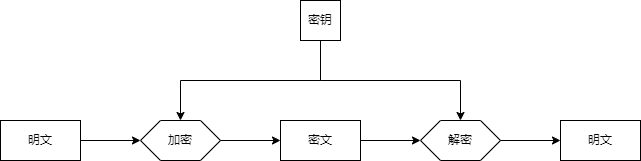
\includegraphics[width=0.8\textwidth]{Picture/Symmetric.png}
    \caption{对称密码加解密过程}
\end{figure}
在分类上,对称密码可以分为流密码(又称序列密码)和分组密码,
\section{流密码}
\section{分组密码}

\newpage
\chapter{非对称密码}
非对称密码指的是加密和解密使用不同密钥的密码算法,其加解密过程大致如下图所示:\par
\begin{figure}[h]
    \centering
    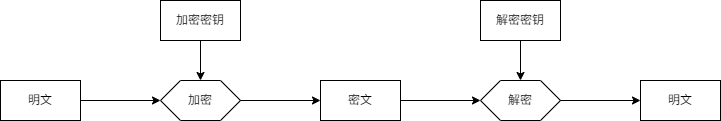
\includegraphics[width=0.8\textwidth]{Picture/Asymmetric.png}
    \caption{非对称密码加解密过程}
\end{figure}\par
上图中加密密钥与解密密钥不相同,在加密密钥和解密密钥之中必有一个是公开的,另一个是保密的,一般称公开的密钥为公钥,保密的密钥为私钥,故有时候非对称密码也被称为公钥密码.\par
在CTF比赛中常见的非对称密码有RSA、ECC(Elliptic Curve Cryptography)等,其中RSA是CTF中最常见且最基础的非对称密码算法.
\section{RSA}
RSA算法是由Ron Rivest、Adi Shamir以及Leonard Adleman三人于1977年提出的非对称加密算法,其安全性基于大数分解的困难性,一般情况下,RSA算法的加解密步骤如下:\\
\textbf{加密}:\par
\begin{enumerate}
    \item 选择两个大质数$p,q$,计算$n=pq$,以及$n$的欧拉函数$\varphi(n)=(p-1)(q-1)$;
    \item 选择一个整数$e$(一般选取$e=65537$),使得$1<e<\varphi(n)$且$(e,\varphi(n))=1$;
    \item 计算$d$使得$ed\equiv 1\pmod{\varphi(n)}$,即$d$是$e$关于模$\varphi(n)$的乘法逆元;
    \item 对于明文$m$,计算密文$c$,即$c\equiv m^e\pmod{n}$;
    \item 将公钥对$(n,e)$公开,私钥对$(n,d)$保密.
\end{enumerate}
\textbf{解密}:\par
\begin{enumerate}
    \item 对于密文$c$,通过私钥$(n,d)$计算明文$m$,即$m\equiv c^d\pmod{n}$.
\end{enumerate}
RSA算法的安全性基于大数分解的困难性,在一般情况下,我们已知公钥$(n,e)$的时候,是很难通过分解$n$得到$p,q$,从而计算出私钥$d\equiv e^{-1}\pmod{\varphi(n)}$的.\par
实际上在CTF比赛中,出题人提供的RSA加密算法往往是有一定的缺陷的,在本节中,我们将主要介绍一些基础的对RSA算法的攻击手段.
\subsection{直接分解模数$n$}
尽管先前提到RSA算法的安全性基于大数分解的困难性,但是在CTF比赛中,RSA加密过程中选取的素数$p,q$可能较小,或者生成的质数存在某些特殊性质,从而导致直接分解$n$变得可行,常见的分解方法有如下几种:
\subsubsection{采用工具分解}

在CTF比赛中,RSA加密过程中生成的质数可能会比较小,抑或者质因数分解结果被人为地加入了某些数据库中公开,这种情况下,我们可以直接使用一些工具来尝试分解模数$n$,常见的工具有factordb(http://www.factordb.com/)、yafu等.\par
factordb是一个在线的质因数分解数据库,对于一个数$n$,我们可以尝试在factordb中搜索$n$,若数据库中存在该数的分解结果,则可以将其用于求解RSA,举个例子,对于$n=463901$,我们可以在factordb上搜索这个数:\\
\begin{figure}[h]
    \centering
    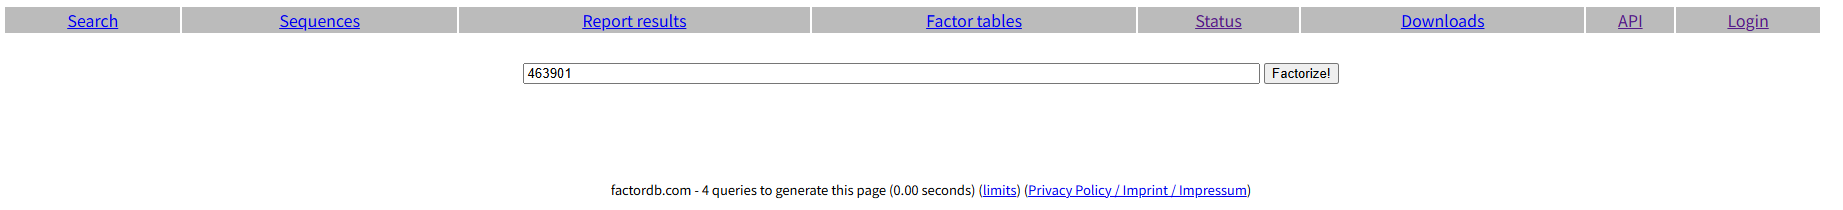
\includegraphics[width=0.8\textwidth]{Picture/factordb_search.png}
    \caption{使用factordb搜索$463901$的质因数}
\end{figure}\\
搜索可以得到如下结果:\\
\begin{figure}[h]
    \centering
    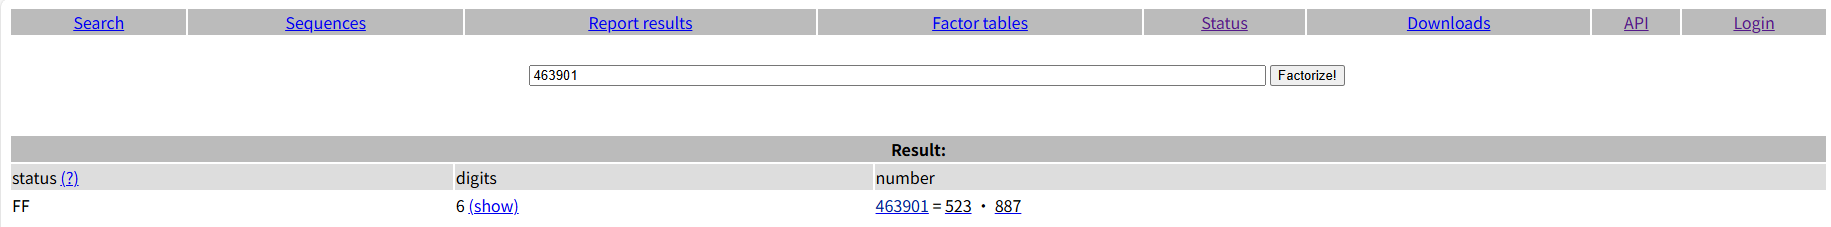
\includegraphics[width=0.6\textwidth]{Picture/factordb_result.png}
    \caption{factordb搜索结果}
\end{figure}\\
此时我们可以得到$463901$的质因数分解结果为$523\times 887$.但是并非所有的数都能在factordb中找到分解结果,若factordb中没有该数的分解结果,对于下面这个由两个512 bits的质数相乘得到的大整数$n$:\\
\begin{figure}[h]
    \centering
    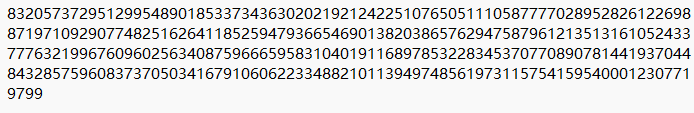
\includegraphics[width=0.8\textwidth]{Picture/ABigNumber.png}
    \caption{两个512 bits的质数相乘得到的大整数$n$}
\end{figure}\\
此时我们尝试使用factordb搜索该数,会得到如下结果:\\
\begin{figure}[h!]
    \centering
    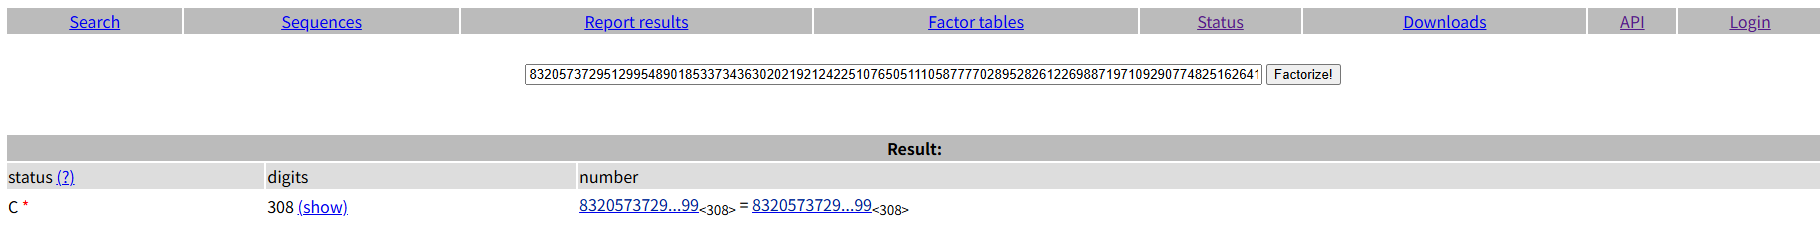
\includegraphics[width=0.8\textwidth]{Picture/factordb_factor_not_found.png}
    \caption{factordb无法搜索出结果}
\end{figure}\\
显然,factordb无法搜索出该数的分解结果,一般在求解RSA问题的时候遇到这种情况就说明我们可能需要采用其它的方法来求解这道RSA问题了.\par
如果想要更方便地使用factordb来分解,我们可以通过Python调用其API来实现自动化分解,有开发者利用factordb的API开发了一个名为factordb-python的库,安装方式可以参考\href{https://pypi.org/project/factordb-python/}{factordb-python},
举个例子,我们以LitCTF 2023中\href{https://www.nssctf.cn/problem/3893}{factordb}题目为例,题目给出如下数据:
\begin{lstlisting}[language=Python,basicstyle=\ttfamily,breaklines=true,keywordstyle=\bfseries\color{blue}]
e = 65537
n = 87924348264132406875276140514499937145050893665602592992418171647042491658461
c = 87677652386897749300638591365341016390128692783949277305987828177045932576708
\end{lstlisting}
那么我们可以通过factordb-python库来分解模数$n$,代码如下:
\begin{lstlisting}[language=Python,basicstyle=\ttfamily,breaklines=true,keywordstyle=\bfseries\color{blue}]
from Crypto.Util.number import *
from factordb.factordb import FactorDB # 导入factordb-python库

e = 65537
n = 87924348264132406875276140514499937145050893665602592992418171647042491658461
c = 87677652386897749300638591365341016390128692783949277305987828177045932576708

f = FactorDB(n) # 创建factordb对象
f.connect() # 连接到factordb
factors = f.get_factor_list() # 获取质因数列表

p = factors[0]
q = factors[1]

phi = (p - 1) * (q - 1)
d = inverse(e, phi)
m = pow(c, d, n)

print(long_to_bytes(m))
\end{lstlisting}
运行代码即可得到flag.\par
除factordb之外,我们还可以使用yafu等工具来分解模数$n$,yafu是一个开源的质因数分解工具,支持多种分解算法,下载地址\href{https://sourceforge.net/projects/yafu/}{https://sourceforge.net/projects/yafu}.\par
这个工具需要通过命令行来使用,对于给定的整数$n$,我们可以在yafu目录下的命令行中输入\texttt{yafu-x64.exe factor(n)}(其中n在实际使用中换成一个具体的数),例如对于先前的$n=463901$,我们可以在yafu目录下的命令行中输入\texttt{yafu-x64.exe factor(463901)},得到如下图所示结果:
\begin{figure}[h!]
    \centering
    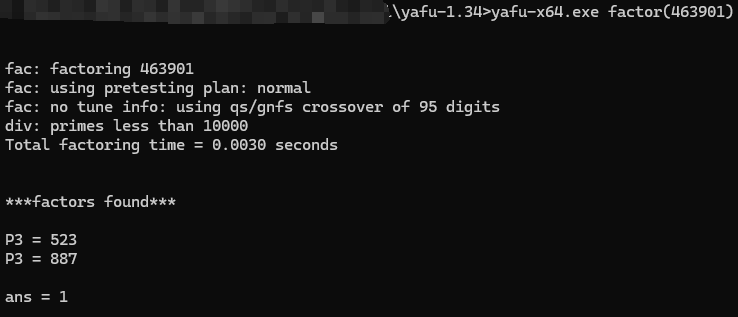
\includegraphics[width=0.45\textwidth]{Picture/yafuFactor1.png}
    \caption{yafu分解结果}
\end{figure}\\
如果要分解的数很大,则不能直接使用\texttt{factor(n)}命令,否则会出现如下图所示的错误:
\begin{figure}[h!]
    \centering
    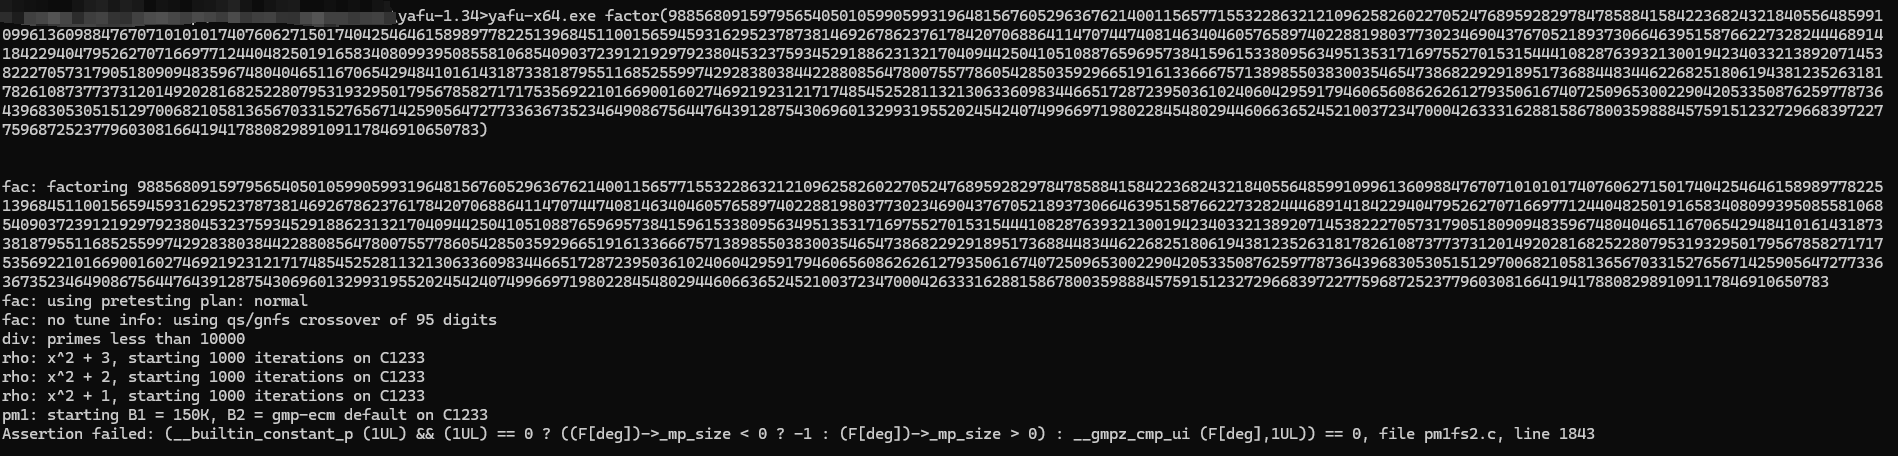
\includegraphics[width=0.8\textwidth]{Picture/yafuFactor2.png}
    \caption{长度过长无法直接分解}
\end{figure}\\
对于这种情况,我们需要先将这个数写入一个文本文件中(例如将其存入n.txt中,注意,数的末尾应有换行),然后在命令行中使用\texttt{yafu-x64.exe "factor(@)" -batchfile n.txt}命令来分解,具体流程在此不过多赘述.

\newpage
\begin{thebibliography}{99}
    \bibitem{1} Joseph H. Silverman. 数论概论(第四版)[M]. 北京:机械工业出版社, 2020.
    \bibitem{2} 闵嗣鹤, 严士健. 初等数论(第四版)[M]. 北京:高等教育出版社, 2020.  
    \bibitem{3} 张苍. 九章算术[M]. 邹涌,译解. 重庆:重庆出版社, 2016.
    \bibitem{4} Michael O Rabin. Probabilistic algorithm for testing primality[J]. \textit{Journal of Number Theory}, 1980, 12(1):128-138.
    \bibitem{5} 杨子胥. 近世代数(第四版)[M]. 北京:高等教育出版社, 2020.
    \bibitem{6} Christof Parr, Jan Pelzl. 深入浅出密码学——常用加密技术原理及应用[M]. 马小婷,译. 北京:清华大学出版社, 2012.
\end{thebibliography}
\end{document}

